\documentclass[british]{article}

\usepackage[british]{babel}% Recommended
\usepackage{csquotes}% Recommended

\usepackage[sorting=nyt,style=apa]{biblatex}

\addbibresource{C:/Users/Daniel/Documents/BibTex/library.bib}

\usepackage[margin=1in]{geometry}
\usepackage{appendix}
\usepackage{amsmath}
\usepackage{graphicx}
\usepackage{listings}
\usepackage{enumerate}
\newcommand{\code}[1]{\texttt{#1}}
\newtheorem{defin}{Definition}
\newtheorem{prop}{Proposition}
\newtheorem{col}{Corollary}
\newtheorem{thm}{Theorem}
\setlength{\parskip}{1em}
\usepackage{placeins}
\usepackage{color}
\usepackage{booktabs}
\DeclareLanguageMapping{british}{british-apa}

\title{CS5014, P2 - Classification}
\author{170008773}
\date{\today}
\begin{document}
	\maketitle
	
	\section{Introduction}
	\label{intro}
	For this assignment, a system to classify certain colours from their optical reflectance spectroscopy readings for both binary and multiclass labelled data was to be implemented. Several methods of classification will be discussed, including Logistic Regression, AdaBoost, Random Forests, Gradient Boosting and Decision Tree with the Decision Tree performing the best. The models were measured on their performance using $k$-fold cross-validation to select a model. After the model selection, the chosen model was re-trained and re-evaluated on the test data and scored using the $F_1$ metric. Finally, the model was being trained on the whole data set to provide a mechanic for classifying previously unseen data.  In the end, the Decision Tree performed best, finally achieving an $F_1$ score of 1.0 on both data sets. 
	
	
	\section{Data preperation}
	\paragraph{Data description} The data consisted of a binary set and a multiclass set. There were 180 samples in the binary set and 450 samples in the multiclass set. Both sets also had 921 features. All of the features consist of intensity readings from the light reflecting off the surface at certain wavelengths.   
	
	\paragraph{Data seperation} Since the data dit not arrive in separate training and testing sets, it had to be seperated first into a testing and a training set. Even though the data contains many of features, the number of samples was relatively low. This meant that not much of the data could be set aside for testing, but it still had to be large enough for the results to be representable. Eventually 25\% of the data was set aside for testing. This was sligtly below a common rule of thumb of setting aside 30\% of the data for testing. 
	
	\paragraph{Normalisation} After the data was separated, it was deemed favourable to normalise the data so that the scale wouldn't introduce additional biases during the rest of the process. A standard normalisation was applied to both the training and test data, according to the values of the training data. 
	
	\section{Initial exploration}
	
	
	\paragraph{Getting a baseline}A data set of these proportions is extremely hard to visualise effectively. Therefore a simple \code{LogisticRegression} classifier was used on the data to get a baseline accuracy. This was done to get a general sense of how complex the data was. If the accuracy of such a simple classifier with no additional work was very high it would suggest that the data was not very complex and that some of the data could probably be pruned. If this was the case then models which could provide more information than just accurate classifications would have to be considered. On the other hand, if this baseline was very low then this would have suggested that the data was very complex and more sophisticated methods with a bigger emphasis on accuracy would have to be considered. The logistic regression classifier achieved an $F_1$ score of 1.0 on both the binary and multiclass data, meaning that it achieved perfect accuracy (for a deeper discussion of why $F_1$ was chosen, see section \ref{metrics}).
	
	
	\paragraph{Moving beyond the baseline} The fact that the baseline accuracy was so high suggests that the data was not very complex and that significant parts could be pruned without a significant loss in accuracy. This is favourable because it allows future data to be stored more compactly and decreases operation time for classifying new data. Therefore, models that provide some mechanic to rank the features in terms of importance were considered, instead of models that would merely provide the best performance. 
	
	
	\section{Model evaluation setup}
	\paragraph{Model selection process} Because it was a goal to provide a mechanic whereby new data could be classified, a model had to be selected. It was decided to use $k$-fold cross-validation to select the model. After a model was selected, it would be trained on all the train data and evaluated on the test data. If this provided satisfactory accuracy then the model would be trained on all available data and then used to predict the previously unseen data. 
	
	\subsection{Cross validation} As previously mentioned it was decided to select a model based on its performance on $k$-fold cross-validation. Special care had to be taken to select an appropriate $k$ for this process. If the $k$ had been too small there would not have been enough folds to make the results representative, but if the $k$ was too large, each of the metrics of each individual fold would not be representative. Eventually $k$ was chosen to be 3 in the binary case and 5 in the multiclass case. This means that each fold would contain 60 samples in the binary case and 90 in the multiclass case which was deemed to be a good distribution. It is important to note that the multiclass folds should be larger than the binary ones since that data is potentially more complex. 
	
	\subsection{Metrics}
	\label{metrics} 
	
	\paragraph{Accuracy}From the baseline measurements, it was clear that more metrics than simple accuracy would have to be considered. For our accuracy, the ubiquitous $F_1$ score, which is the so-called `Harmonic mean', of the precision and the recall, was used with micro averaging in the multiclass case. This, in theory, means that the $F_1$ score measures both recall and precision at the same time, valuing both equally. $F_1$ is defined as $$F_1 = \frac{2}{\frac{1}{recall} + \frac{1}{precision}} = \frac{2\cdot TP}{2\cdot TP + FP + FN}$$ Where $TP, FP, FN$ represent the number of true positives, false positives and false negatives respectively \autocite{Lipton2014}. Firstly, $F_1$ was chosen because of its ubiquity. Reasons to choose other metrics could have been that either recall or precision could have been deemed more important, but this was not believed to be the case given the context. Secondly, $F_1$ was initially used in the baseline measurement because it was the default way to measure accuracy in sci-kit learn \autocite{Pedregosa2012}. After it was used in the baseline measurement it became clear that the accuracy was already perfect and thus it wouldn't have made sense to use other metrics that favour or punish mistakes differently. The micro averaging is the most accurate metric that is mentioned by \citeauthor{Lipton2014} and was therefore deemed to be the most favourable to use. 
	
	\paragraph{Beyond accuracy} As mentioned before, the accuracy of the baseline suggested that more metrics than simple accuracy would have to be considered. Beyond accuracy, two other metrics were deemed relevant namely the number of features the algorithm could reduce the full data set too and the total operation time. It was deemed desirable to have a single numerical metric on which to base the model selection since that would make the decision process easier to automate, and more generally applicable. For this reason a metric defined as $\frac{\mu_s}{T}$ was used. Here $\mu_s$ represents the mean score on the training sets across all cross-validation folds and $T$ represents the total time of operation on the feature set, i.e. the time spent both training and testing across all folds. A higher rating in this metric is considered to be better. This metric was considered because it would allow, for example, for models to be selected that might have slightly less than perfect accuracy but performed orders or magnitude faster than the rest, which was deemed to be desirable. This metric also implicitly takes into account the number of features, since if the model can perform its classification with less features, it will generally do so in less time. It should also be noted that this metric says much about the performance of the models in isolation and is only intended for comparing models.
	
	The astute reader might remark that this metric has some sensitivity issues. For example, a classifier that performs poorly but does it in fractions of microseconds would do quite well even though this is not the desired behaviour. This was not deemed to be a problem in this context, however, because the baseline measurement already suggested that the accuracy of all the models would be similar, i.e. near perfect. Therefore these sensitivity issues would not distort the results. It was also verified manually that this metric performed as expected. 
	
	\subsection{Models} As mentioned before, models that provide some mechanic of ranking features in terms of importance were to be considered. It was decided to try a variety of different methods namely: Logistic Regression, Gradient Boosting, Random Forests, Decision Tree and AdaBoost. All of these models, except Logistic Regression, provide native mechanics of ranking features according to their impact. For Logistic Regression, Recursive Feature Elimination (RFE) was used. 
	
	
	\section{Evaluating the model}
	\label{evaluation}
	The results of the $k$-fold cross validation runs for the binary and the multiclass data can be found in Figure \ref{binaryTable} and \ref{multiclassTable} respectively. 
	\begin{figure}
		\begin{tabular}{|l|rrrrr|}
			\toprule
			Algorithm &  Mean score &  Total operation time & Important features & Feature set &      Rating \\
			\midrule
			Decision tree &         1.0 &              0.003655 &                            1 &     reduced &  273.618892 \\
			Adaboost &         1.0 &              0.008293 &                            1 &     reduced &  120.581417 \\
			Logistic regression &         1.0 &              0.019660 &                          460 &     reduced &   50.864093 \\
			Decision tree &         1.0 &              0.026309 &                            1 &        Full &   38.010476 \\
			Adaboost &         1.0 &              0.031199 &                            1 &        Full &   32.051842 \\
			Random Forests &         1.0 &              0.049511 &                           10 &     reduced &   20.197355 \\
			Logistic regression &         1.0 &              0.050313 &                          460 &        Full &   19.875675 \\
			Random Forests &         1.0 &              0.055884 &                           10 &        Full &   17.894246 \\
			Gradient Boosting &         1.0 &              0.131196 &                           70 &     reduced &    7.622168 \\
			Gradient Boosting &         1.0 &              0.841714 &                           70 &        Full &    1.188051 \\
			\bottomrule
		\end{tabular}
		
		\caption{A table containing the metrics of the models using $k$-fold cross validation on the binary data set, in order of decreasing rating}
		\label{binaryTable}
	\end{figure}
	\begin{figure}
		\begin{tabular}{|l|rrrrr|}
			\toprule
			Algorithm &  Mean score &  Total operation time & Important features & Feature set &      Rating \\
			\midrule
			Decision tree &    0.997015 &              0.005924 &                            4 &     reduced &  168.301352 \\
			Random Forests &    1.000000 &              0.087713 &                           41 &     reduced &   11.400849 \\
			Random Forests &    1.000000 &              0.148290 &                           41 &        Full &    6.743536 \\
			Decision tree &    0.991000 &              0.291626 &                            4 &        Full &    3.398190 \\
			Linear &    1.000000 &              0.357316 &                          460 &     reduced &    2.798647 \\
			Adaboost &    0.807071 &              0.674922 &                           43 &     reduced &    1.195799 \\
			Linear &    1.000000 &              0.852753 &                          460 &        Full &    1.172672 \\
			Gradient Boosting &    0.994198 &              2.261343 &                           88 &     reduced &    0.439649 \\
			Adaboost &    0.903337 &              6.247627 &                           43 &        Full &    0.144589 \\
			Gradient Boosting &    0.988137 &             13.692962 &                           88 &        Full &    0.072164 \\
			\bottomrule
		\end{tabular}
		
		\caption{A table containing the metrics of the models using $k$-fold cross validation on the multiclass data set, in order of decreasing rating}
		\label{multiclassTable}
	\end{figure}
	
	\section{Discussing the results}
	\label{discussion}
	\subsection{Model performance}
	\subsubsection{Binary}  In the binary case all the models achieved perfect accuracy on both the full and the reduced feature set. Here the Decision Tree still won by quite a significant margin over its closest competitor AdaBoost. Both the models were able to reduce the feature set down to 1, but the Decision Tree was faster. After being retrained on all the training data the Decision Tree achieved an $F_1$ score of 1.0 on the test data (i.e. perfect accuracy). This would imply that this classification method would certainly be useful in any application where data like this is to be used, assuming that the provided data was representative. Accuracies like these are, by and large, considered to be unreasonable to attain, and this might raise some concern over whether the data used was representative, but that discussion is outside the scope of this assignment.  
	
	\subsubsection{Multiclass} The Decision Tree also performs best on the multiclass set. Even though it does not achieve perfect accuracy on the multiclass set, it does this in an order of magnitude less time than its closest competitor (the random forest on the reduced set) and reduces the feature set to 4 instead of the 42 the random forest achieved, meaning that manual analysis can be performed on that feature set much easier. This was exactly the reason that the rating metric described in section \ref{metrics} was chosen.
	
	\paragraph{Speed vs accuracy}  In mission-critical applications, such as medical or military operations, perfect accuracy might be deemed more important than speed, in which case the random forest would have been preferable, but this was not the case for this research. It is of course also true that speed performances beyond a certain point do not matter. When the classification time no longer is the bottleneck in the system operation, improving the speed further does not help. This, however, is too context specific to be discussed here. This also makes the automatic rating a lot more complicated so this would have to be done manually or would require more research into more sophisticated ranking metrics.  
	
	\paragraph{Stability of the accuracy} It should also be noted that the models used are largely stochastic, this means that the accuracy they achieve might not be completely equal across runs. This is especially true in the multiclass case. This is not a cause for concern however as they should be largely stable, which was manually verified to be true. This is also partially true due to the fact that the data set contained relatively few samples. 
	
	\paragraph{AdaBoost performance} It is interesting to note that on the binary set AdaBoost outperformed the Random Forsts and on the multiclass set this order was reversed. Consider that while Decision Tree is very effective here, it generally isn't considered to be extremely robust. Other ensemble methods like AdaBoost cater more for noisier data. AdaBoost is a somewhat old algorithm \autocite{Freund1997} and there have been newer iterations of this algorithm \autocite{NormalHedge, Otten2016, Vente2016}. It might be that these newer versions could perform better, while also being more robust.  
	
	\paragraph{Final performance of the Decision Tree}After being retrained on all the trainings data the Decision Tree achieved an $F_1$ score on the test data (i.e. perfect accuracy). This would imply that this classification method would certainly be useful in any application where similar data used, assuming that the provided data was representative. Accuracies like these are by and large, considered to be unreasonable to attain, and this might raise some concern over whether the data used was representative, but that discussion is outside the scope of this assignment.
	
	\subsection{Feature importance and analysis}
	
	\begin{figure}[!ht]
		\centering
		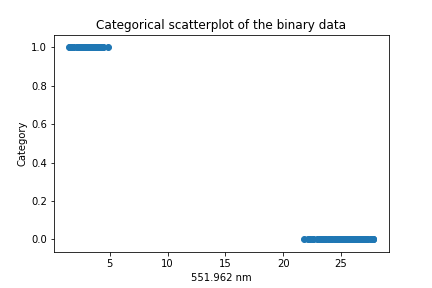
\includegraphics[width=0.5\textwidth]{binaryScatterplot}
		\caption{A scatter plot of the category vs the best feature of the binary data set}
		\label{binaryScatterplot}
	\end{figure}
	
	\paragraph{Binary} Looking at figure \ref{binaryScatterplot} confirms that indeed the data is not extremely complex. When looking at this feature it is easy to see that the data is linearly separable. This explains how even the logistic regression could achieve perfect accuracy. It should be noted however that it was because of the mechanics of the Decision Tree that this feature was found. Another interesting note is that the feature used is not stable over runs, meaning that there are multiple features that exhibit this separability characteristic.    
	
	
	
	\begin{figure}[!ht]
		\centering
		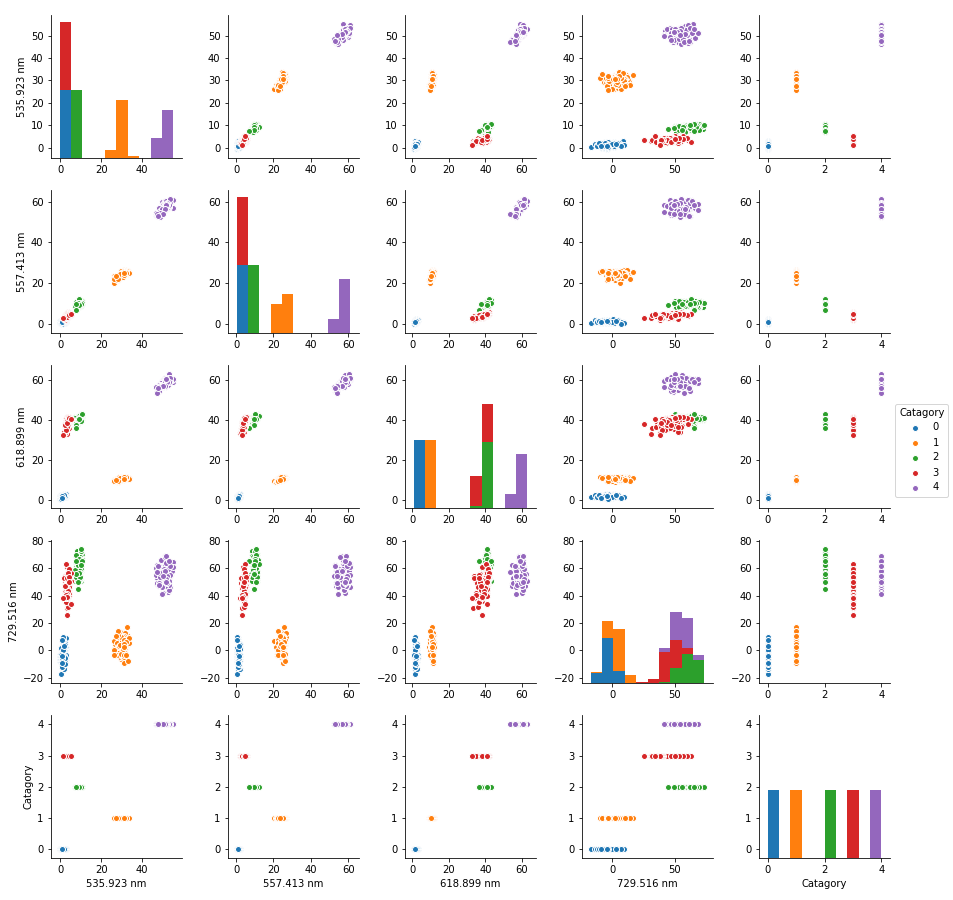
\includegraphics[width=\textwidth]{multiclassScatterplot}
		\caption{A scatter plot matrix of the best features of the multiclass data set}
		\label{multiclassScatterplot}
	\end{figure}
	
	
	\paragraph{Multiclass} Looking at the scatterplot matrix of the 4 features extracted by the Decision Tree, it becomes clear that the multiclass set is somewhat more complex but still relatively simple. Most of the scatter plots exhibit a high degree of separability. Again it should be noted that the features used are not completely stable over runs. This means that there are multiple feature sets that exhibit the separability shown in the figure. Due to the stochastic nature of the models used and the relatively low amount of available data, the Decision Tree can sometimes select different features resulting in slightly less accuracy. Whether this constitutes cause for concern is left for the reader to decide. If this is the case, the random forest would be preferable, as that model is more reliable, though slightly slower. Again, this might not make a difference if the model operation is no longer the bottleneck in the system.     
	
	\subsection{Limitations}
	The conclusions of this study are very limited in scope. Only standard out-of-the-box models were considered, although given the performance achieved this is not a cause for concern. So too, the amount of data available was less than ideal and the data itself was extremely specific and clean, making the results in this study less widely applicable. Furthermore, the possibly uncanny performance could raise concerns over whether the data used was actually representative. One could reasonably postulate that this study has not explored measures of robustness very well and thus if future data proved to be more noisy that could cause trouble.
	
	
	word count:  2299
	\FloatBarrier
	\printbibliography

	\begin{appendices}
	\section{Binary classification result}
	\label{binary}
	\lstinputlisting{../binaryTask/PredictedClasses.csv}
	
	\section{Multiclass classification result}
	\label{multiclass}
	\lstinputlisting{../multiClassTask/PredictedClasses.csv}
\end{appendices}
\end{document}
